\begin{artengenv}{Marek Ku\'s}
	{No-signaling in topos formulation and a common ontological basis for classical and non-classical physical theories}
	{No-signaling in topos formulation and a common ontological basis\ldots}
	{No-signaling in topos formulation and a common ontological basis for classical and non-classical physical theories}
	{International Center for Formal Ontology,\\
	Warsaw University of Technology}
	{Starting from logical structures of classical and quantum mechanics we reconstruct the logic of so-called no-signaling theories, where the correlations among subsystems of a composite system are restricted only by a simplest form of causality forbidding an instantaneous communication. Although such theories are, as it seems, irrelevant for the description of physical reality, they are helpful in understanding the relevance of quantum mechanics. The logical structure of each theory has an epistemological flavor, it is based on analysis of possible results of experiments. In this note we emphasize that not only logical structures of classical, quantum and no-signaling theory may be treated on the same ground but it is also possible to give to all of them a common ontological basis by constructing a ``phase space'' in all cases. In non-classical cases the phase space is not a set, as in classical theory, but a more general object obtained by means of category theory, but conceptually it plays the same role as the phase space in classical physics.}
	{none.}




\lettrine[loversize=0.13,lines=2,lraise=-0.03,nindent=0em,findent=0.2pt]%
{O}{}ntological assumptions of classical and quantum picture of the world differ significantly, despite the fact that both description attempt to grasp the structure of the same reality. The fact that they offer a glance from two different points of view---macroscopic and microscopic, should not interfere with a pragmatic request that, at least to compare both theories, we should have in both some common `elements of reality', e.g. some observables that pertain to the same physical quantities on both level, like `position', `momentum', `angular momentum' etc. An alternative (let's call it Kuhnian) approach would be to deny connections between concepts used in both theories pointing to (seemingly) the same properties of physical systems, (e.g.\ Newtonian and Einsteinian mass \parencite{kuhn_structure_1970}). The latter approach is not particularly attractive from the point of view of a practicing physicist. It leaves no room for many useful and fruitful procedures as e.g., a `semiclassical/classical approximation'.

Classical systems are described in terms of a phase space, usually a differential manifold with some additional (symplectic/Poisson metric) structures. Observables, i.e.\ physical quantities that we can measure, or, in general to which we can ascribe certain numerical values characterizing the observed system, are functions on the phase space.
Values of observables, like positions, momenta, energies, angular momenta etc., are some intrinsic properties of physical systems (particles, ensembles of particles, rigid bodies, etc.). They can change in time, but are properties that are possessed by systems alone and do not depend on whether or not they are actually measured at a particular moment. At least in principle, we can measure them without disturbing them. Consequently, measurements can be performed in an arbitrary order, or even simultaneously, and provide the same results. We can thus pose questions about \textit{exact} values of, say, the position and the momentum of a particle. Usually, however, due to e.g. inaccuracies of measurements we inquire into the probability  that our particle is in a certain subset of the phase space. Such a probability is determined by the volumes of the relevant subsets. Physical states can thus be identified with probability distributions on (measurable) subsets of the phase space. Mean values (results of experiments) can be calculated using these distributions.

% Among them we can distinguish elementary ones that can be identified with questions whether a phase-space points characterizing a physical, (\textit{via}, e.g., value of the position and momentum), belongs to a particular subset of the phase space. Finally, 

In quantum mechanics we do not have a clear notion of a `phase-space' in the form of a manifold. A backbone structure is provided by a Hilbert space $ \mathcal{H} $, observables are identified with self-adjoined operators, and states with non-negative, trace-class operators (density states). We may ascribe to each system some properties that pretend to be quantum analogues of classical ones, like positions, momenta, angular momenta, energies, etc.\ (and some others that seem to be of a purely quantum mechanical nature, like spin, isospin, strangeness, hypercharge etc.). However, they are no longer \textit{intrinsic} in the classical sense. They are not `carried' by a system during its evolution, rather they are `brought to life' by an act of measurement.
         
         
Hence, it is hard to find a unifying ontological basis for classical and quantum physics. Fundamental elements of physical reality, as positions, momenta, angular momenta, etc. have different ontological status in both theories. For everyday physical practice this does not pose any clear and present danger. Ultimately, physics is an experimental science. It aims at answering experimental questions about outcomes of measurements putting emphasis on the epistemology, at the price of moving apart, or even totally discarding ontological issues.  
         
%The ontological differences between quantum and classical descriptions of the physical world are well reflected on the mathematical level.   

     
%In quantum mechanics  Each act of measurement disturbs the actual state of a system by bringing it to another state corresponding to a result of the measurement performed. Hence, the order in which measurements are taken  does matter, and some measurements can not be taken  simultaneously (the uncertainty principle). Moreover, although results of measurements depend on the actual state of the system prior to the act of a measurement, they do it only in  a probabilistic manner. For each observable (position, momentum, angular momentum, energy, spin, etc.), there is a corresponding selfadjoint operator, the eigenvalues of which are possible outcomes with probabilities depending on the state of a system before the measurement and the eigenvectors determine possible states after it.   

An attempt to unify classical and quantum physics on common epistemological ground goes back to Birkhoff and von Neumann \parencite*{birkhoff_logic_1936} in form of the so-called quantum logic. The main idea is to analyze the structure of elementary experimental question/propositions about a system. In classical physics, elementary propositions can be reduced to statements that values of observed quantities (positions, momenta) belong to a certain subset of the phase space. The logical structure of the set of such propositions, determined by the rules concerning their negations, conjunctions and disjunctions, isomorphically reflects the Boole algebra structure of the set of (measurable) subsets of  the phase space. One of the fundamental features of the resulting lattice\footnote{A partially ordered set in which every two elements have a unique supremum---the set-theoretical sum on the level of subsets and conjunction on the level of proposition, and infimum---the  set-theoretical intersection of subsets and disjunction, respectively.} is the distributivity law, allowing for the distribution of conjunctions over disjunctions and \textit{vice versa}.  

In quantum mechanics elementary propositions concern positions of state vectors (characterizing a state of a system) with respect to eigenspaces of observables. As in the classical case we can ask composite questions corresponding to conjunctions and disjunctions. However, the ensuing logical structure is no longer distributive. The logic of a system described by a  Hilbert space $\mathcal{H} $ is represented by the orthomodular lattice of  closed subspaces in $\mathcal{H}$. The involution sending a subspace to its  orthogonal complement represents logical negation, still as in the classical case, satisfies  the law  of an excluded middle: measuring the spin of an electron will yield either `up' or `down'. The  resulting lattice is, however,  non-distributive: $x$-spin up does not imply $x$-spin up and  $z$-spin up or $x$-spin up and $z$-spin down. Having the lattice stand for the logic of the system, one derives its probability theory, where  states assign probabilities to elements of the lattice, respecting the underlying structure (order and complementation). These states turn out to coincide with the usual density matrices by the Gleason theorem \parencite{gleason_measures_1957}.

%The above described approach provides a unifying picture for both theories, classical and quantum with a clearly epistemic flavor. A backbone is constituted by a certain lattice of propositions (experimental questions concerning outcomes of experiments) and the corresponding probability theory. The differences reflect precisely the dissimilarities between the two theories. Still, however, a fundamental ontological question `what there is?', is answered differently by both theories. In classical mechanics values of observables (dependent on the actual state of a system) are intrinsic properties of systems (they exist `objectively' i.e they are "intrinsic properties" of systems) and  probabilistic features (if they are relevant) are due to lack of precise knowledge of the actual state of a system. In the quantum setting values of observables (dependent on the actual state of a system) become determined by measurements performed on a system, i.e. they are not "intrinsic properties" of systems and the probabilistic character of the theory is due to "intrinsic (ontic) randomness" \parencite{bera17}.

Having two examples of different theories pertaining to the same physical reality, we are tempted to think about other similar constructions. From what we know now, it is hard to construct a successful theory that e.g., supersedes quantum mechanics \parencite{aaronson_is_2004}. Instead we can identify some common epistemic structures in classical and quantum mechanics encoded in logics of both theories, i.e. the logical structures of the sets of their propositions, and try to construct similar, reasonable theories.

One of such attempts was presented by Popescu nad Rohrlich \parencite*{popescu_quantum_1994} in the form of so called no-signaling boxes. They started from a paradigmatic correlation experiment, that can be performed both on classical and quantum level depicted schematically in Fig.\ref{fig:bellex1}. The model is supposed to describe the most elementary system composed of two separated subsystems. We can think of inputs as observables that we choose to measure, and outputs as the results of measurements. In the simplest case we have two observables, encoded (labeled) by $0$ and $1$, each of which can take two values $0$ and $1$. Performing multiple measurements we will obtain a sequence of outcomes allowing us to determine the relative frequency $P(\alpha\beta| ab)$ of getting any pair of outputs $\alpha\beta\in  \{0, 1\}\times \{0, 1\}$, given any pair of inputs $a b \in  \{0, 1\}\times \{0, 1\}$.

In order to have a legitimate interpretation of $P: \{0, 1\}\times \{0, 1\}\times \{0, 1\}\times \{0, 1\}\rightarrow \mathbb{R}$ in terms of probability, it should fulfill the following requirements,
\begin{enumerate}
	\item $ 0\le P(\alpha\beta| ab)\le 1 $ (positivity),
	\item $ \sum_{\alpha\beta}P(\alpha\beta| ab)=1 $ (normalization),
	\item $ \sum_\alpha P(\alpha\beta| ab)=\sum_\alpha P(\alpha\beta| cb)  $; $ \sum_\beta  P(\alpha\beta| ab)=\sum_\beta  P(\alpha\beta| ac)  $ (no-signaling).
\end{enumerate}
The last property, non-signaling, is supposed to encode the principle of relativistic causality, i.e.\ what happens in one box does not influence the other obeyed by spatially separated subsystems. We will refer to this particular example of non-signaling boxes as the (2, 2)-box world.

\begin{figure}
	\centering
	\includegraphics[width=0.7\linewidth]{ART_Kus/BellEx1}
	\caption{A two-system correlation experiment}
	\label{fig:bellex1}
\end{figure}


%\begin{figure}[h]\label{fig:bellex1}
%	\centering
%	\includegraphics{BellEx1}
%	\caption{Two-system correlation experiment}
%	\label{fig:bellex1}
%\end{figure}
%Such an experimental setup can be easily constructed classically. Quantum-mechanically we can realize it \textit{via} measurements of spins of two spin-$\frac{\mathrm{1}}{\mathrm{2}}$ particles or polarizations of two photons emitted from a common source (an atom) undergoing two consecutive electric dipole transition. Different directions of polarizers or magnets measuring polarizations or spin correspond now to different observables \parencite{peres06}. 
For a particular instance of (2,2)-box world we may postulate concrete values of $P(\alpha\beta| ab)$ fulfilling 1.-3. Popescu and Rohrlich \parencite*{popescu_quantum_1994}  proposed the following,
\begin{equation}\label{PRbox}
P(\alpha\beta|ab) = \bordermatrix{
	\mathrm{} &  xx &  xy &  yx &  yy \cr
	00 & 1/2 & 1/2 & 1/2 &   0 \cr
	01 &   0 &   0 &   0 & 1/2\cr
	10 &   0 & 0   & 0   & 1/2\cr
	11 & 1/2 & 1/2 & 1/2 &   0
}.
\end{equation}    

Usually $P(\alpha\beta| ab)\ne P(\alpha|a)P(\beta|b)$, where $P(\alpha|a)$ and $P(\beta|b)$ are one-particle probability distributions of measurements results of $a$ and $b$. One introduces thus the correlations,
\begin{equation}\label{corr}
\langle ab \rangle = \sum_{\alpha,\beta\in\{0,1\}}\alpha\beta P(\alpha\beta|ab).
\end{equation}
It can be now checked that in the classical and quantum cases the following combination of correlations
\begin{equation}\label{S}
S:=|\langle a_1 b_1 \rangle + \langle a_2 b_1 \rangle + \langle a_2 b_2\rangle - \langle a_1 b_2 \rangle|
\end{equation}
that, in principle, can achieve the maximal value of $4$ (each of the term is not larger than $1$ in absolute value) is further restricted. Classically $|S|\le 2$ (Bell \parencite*{bell_einstein-podolsky-rosen_1964} inequality in the CHSH form \parencite{clauser_proposed_1969}) whereas in quantum mechanics $|S|\le 2\sqrt{2}$ (Tsirelson's bound \parencite{cirelson_quantum_1980}).  
For the Popescu-Rohlich box (\ref{PRbox}) we have $S=4$.

In the quantum logic approach the elementary admissible questions are,
\begin{itemize}
	\item `Does our system belongs to a (measurable) subset of the phase-space?' (classical mechanics);
	\item `Is the result of measuring the projection on a closed subspace of the Hilbert space of the system equal to $1$?' (quantum mechanics);
	\item `Does measuring $a$ on a subsystem gives an outcome $\alpha$?' (Popescu-Rohrlich).\footnote{In fact we should ask about an outcome of a joint measurement of $a$ in the first subsystem and $b$ in the second one.}
\end{itemize}
One can now combine elementary questions by the conjunction and disjunction and negate them. As already said the resulting lattice is a Boolean algebra in the classical case and so-called orthomodular lattice which is non-distributive\footnote{Conjunctions do not distribute over alternatives and \textit{vice versa}.} \parencite{birkhoff_logic_1936}. For the Popescu-Rohrlich box (\ref{PRbox}) allow the appropriate one is that of a so-called orthomodular poset (for details see \parencite{tylec_non-signaling_2015,tylec_ignorance_2018}). The resulting structure has some common features with quantum mechanics, e.g., the truth of the alternative $p\vee q$ of statements $p$ and $q$ does not imply that $p$ is true or $q$ is true (the `Schr\"odinger cat' paradox). Moreover, as in quantum mechanics measurements are, in general, destructive. Performing a measurement changes irreversibly a state of a system and does not allow its exact reconstruction \parencite{tylec_non-signaling_2015}. On the other hand, from some points of view, Popescu-Rohrlich boxes are `more classical' than `quantum mechanical', since  in both theories the Heisenberg uncertainty relations are not fulfilled \parencite{tylec_non-signaling_2015}.   
 
As already emphasized the quantum logic approach has a rather epistemic flavor. We concentrate on learning system properties from observations/measurements. Instead, the category theory seems to provide a path to `restore a common ontology' for all considered theories. One can cast the program into a sequence of goals.

\begin{itemize}
	\item Find a well behaved phase space for quantum and a no-signaling systems. 
	\item Find a logical structure of the set of propositions 
	\item Reproduce the probabilistic properties of the theory.
\end{itemize} 

Since the well understood ontological assumptions of classical theory are, as argued above, connected to the notion of the phase-space, it would be desirable to construct phase-spaces for non-classical theories in such a way that they resemble `as much as possible' the classical one. This opens a possibility to interpret quantum mechanics and no-signaling theories in a realistic sense, like we do it in classical physics, where we can assign truth values to propositions without reference to measurements. Hence, we can maintain that propositions refer to some `real objects' or `real properties' independent of observers and measurements. This is exactly what I call a `restoration of a common ontology' for all theories considered here.    

As it will be clear, we have to be ready to pay some price. The resulting `logic' of a phase-space need not to be a Boolean one, so the \textit{tertium non datur} principle need not to be fulfilled. Nevertheless the probabilities calculated on such a `logic' (just as the probabilities in the classical physics calculated on the Boolean logic of subsets of the phase space) will reproduce quantum mechanical and no-signaling results. Moreover, what separates logics of non-classical theories from the classical one, i.e.\ its non-distributivity, responsible for nearly all `paradoxes' of quantum mechanics (and no-signaling theories) will be avoided.        

For quantum mechanics, this can be done within a program presented by Isham and D\"oring \parencite{doring_topos_2008,doring_topos_2008-1,doring_topos_2008-2,doring_topos_2008-3}, in terms of the category theory or, more specifically, the topos theory. In what follows I will employ a slightly different approach \parencite{wolters_comparison_2013}, using the same mathematical apparatus of categories and topoi, proposed originally by Heunen, Landsman, and Spitters \parencite*{heunen_topos_2009,heunen_gelfand_2011} called `Bohrification'\footnote{For the explanation of the chosen name consult the cited papers of Heunen\textit{ et al.}}. In \parencite{gutt_non-signalling_2016} we extended  the construction  to no-signaling boxes. Finding an analog of a classical phase-space is, in a certain sense, the principal goal. 

Let me shortly describe main mathematical ingredients of the above outlined approach. A category is a structure consisting of `objects' connected by `arrows'. From the definition we may compose the arrows (an arrow from an object to a second one followed by another arrow from the second object to a third one) and the composition is associative. A very intuitive example of a category is the category of sets, $\mathbf{Set}$, where the objects are sets, and the arrow connecting a set $A$ to a set $B$ is a function from $A$ to $B$.\footnote{From the point of view of the category theory $\mathbf{Set}$ is not so trivial, since the collection of its objects is not a set---such a category is called a `large category'. As an example of a `small category' employing sets as objects we can take a category of open subsests of some topological space (`a classical phase-space' in the sense described previously). } A topos is a category with some additional properties chosen in a way that results in a certain generalization of $\mathbf{Set}$. The appropriate formal definition and all needed technical details can be found in one of numerous books on the categories and topoi \parencite[e.g.][]{goldblatt_topoi_2014} will not be invoked here.\footnote{For a clear exposition of applications in quantum physics \parencite{flori_first_2013} and \parencite{flori_second_2018} are, probably, the best choice.} What is important is that basic constructions involving sets, like e.g., exponentiation $A^B$, i.e, the set of all functions from $A$ to $B$, have their equivalents for topoi, and that (from definition) each topos is equipped with the, so-called, sub-object classifier. The latter is a special object of the considered category, the meaning of which can  be understood taking again as an example a set $S$ and its subsets. We can express the fact that $S$ is a subset of $S$ by considering a characteristic function of $A$, i.e., the function from $S$ to the set $\{0,1\}$ which takes the value $1$ on $s\in S$ if $a\in A$ and the value $0$ otherwise. The two-element set $\{0,1\}$ is the `subobject classifier' making $\mathbf{Set}$ a topos. The fact that the subobject classifier is a two-element set (we can refer to value $1$ as `true' and to $0$ as `false') is clearly strictly connected to the Boolean structure of the algebra of subsets (and to the `logic' of a classical phase-space described previously). In general topos the subobject-classifier need not be a two-element set, but some more general object in the category. As a consequence the `logic' of a topos need not be Boolean any longer, but it is a so-called Heyting algebra, which is distributive, but, in general, the principle of excluded middle is no longer valid. A nice example is a lattice of open subsets of a topological space. It is partially ordered by the set-theoretic inclusion and, as in the case of subsets of some set, we have here the ordinary set-theoretical algebraic operations of sum and intersection corresponding to alternative and conjunction, but since the set-theoretical completion of an open set is not open. we have to take the interior of  the completion to achieve the proper representation of negation. But then the principle of excluded middle is not fulfilled, since the sum of an open set and the interior of its interior is not the whole space, in contrast to the case of subsets of a set $S$, where a subset $A$ and its completion $S-A$ sum up to the whole $S$ (\textit{tertium non datur}). Obviously the lattice remains distributive, since sums distribute over intersections and \textit{vice-versa}.

Roughly speaking (some technical refinements are needed to end up with a proper result, see the cited papers of Heunen \textit{et al.}), one finds a well-behaved phase space by constructing an `internal logic' (a Heyting algebra) of some topos and identifying this very topos with the looked-for phase-space. In the construction of Heunen \textit{et al.}, concerning quantum mechanics, the starting point is the set $\mathscr{C}$ of commuting sublagebras (`contexts') of observables on the Hilbert space $\mathcal{H}$ instead of the set of all orthogonal projections acting on it. Each such a context has a well defined physical meaning as a set of compatible measurements. The partially ordered by inclusion set of contexts is treated as a category with contexts as objects and arrows as inclusions. The construction of the 'internal logic' goes through several technical steps (again, for details consult \parencite{heunen_topos_2009,heunen_gelfand_2011}) ending with a topos which is identified with the  'phase-space' we were looking for. In a natural way one defines also states of a systems, and what is most important, a method of calculating probabilities of outcomes of experiments (reproducieng the quantum mechanical results).

 In \parencite{gutt_non-signalling_2016} the above construction was extended to no-signaling boxes. Here we do not have a natural Hilbert space structure as a playground, consequently thus a natural analogue of commuting algebras is lacking. Nevertheless, one can consistently define contexts (situations where measurements are compatible). As a result it was possible to define an appropriate phase-space $\Sigma$, states of the box-world and probabilities on $\Sigma$ reproducing the correlation structure in it.  Hence, in terms of category theory one can `restore the ontology' (phase-space) also for the Popescu-Rorlich boxes. The resulting phase space is, again, not a set, but a more general object, namely a particular topos. Thus all three theories are put on the same level with phase spaces described by appropriate topoi. This suggests a hypothesis that the approach is, in some sense, universal and applicable also to other, possible `generalizations of quantum mechanics' of the whole procedure.
 
 For quantum mechanical systems other approaches of generalizing the classical phase-space descriptions were considered in the past (and are still in use). The most popular employs the classical phase-space parameterized by positions and momenta at the price of lack of possibility to define in a consistent way positive-definite probability functions reproducing quantum mechanical results (using instead so called `quasiprobabilities' like, e.g., the Wigner function). It is not clear how one relates this approach to the topos-theoretic one described above. For no-signaling theories it is even harder, since no starting point (a classical phase-space on which some quasiprobabilities are defined) is easy to identify.    

\end{artengenv}
